\section{Démarche Expérimentale}

Afin de mesurer la viscosité d'un liquide en fonction de la temperature de ce liquide, un viscosimètre est utilisé, shématisé à la \autoref{fig:montage}. Les liquides à étudier sont mis dans des tubes en verre, en \textbf{a} et \textbf{b}. Cestubes sont plongés dans un bain d'eau permettant de chauffer uniformement les liquides étudiés. Une pompe en \textbf{p} permet d'homogéniser la température de l'eau. La température de l'eau est controlée par un corps de chauffe en \textbf{c} et un circuit de refroidissement en \textbf{s}. Un thermomètre pour chaque liquide est utilisé pour connaitre plus précisement la température des liquides.

\begin{figure}[h]
    \centering
    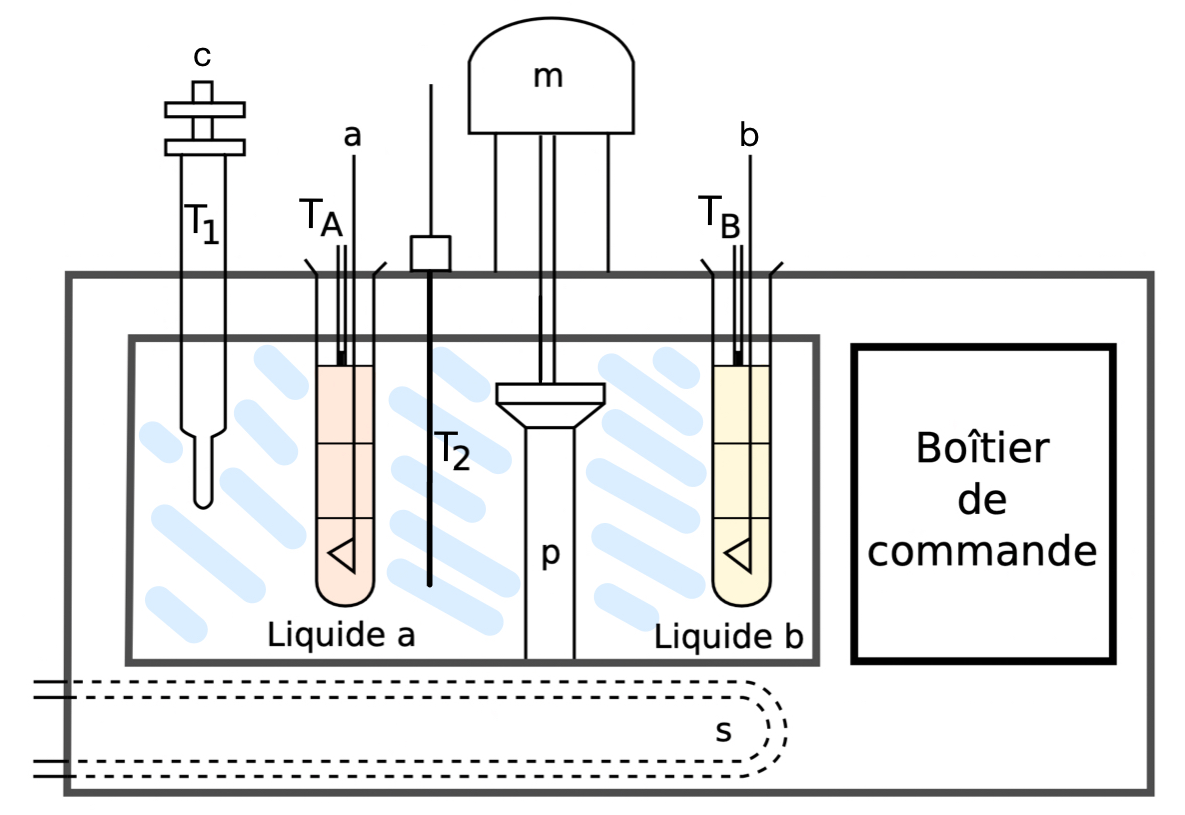
\includegraphics[width=0.8\linewidth]{figures/montage.png}
    \caption{Montage expérimental \cite{notice}}
    \label{fig:montage}
\end{figure}

Pour cetter expérience, deux huiles, HF 16-681 et HF 16-685, qui seront dénotées huile 1 et huile 2, seront étudiées. Une bille de masse et rayon connue est alors lachée à la surface de chaque huile et il est supposé qu'elle atteint sa vitesse maximale \(v_\infty\) avant un premier marqueur. Le temps entre le passage du premier marqueur et du deuxième marqueur est mesuré et permet d'obtenir la vitesse maximale \(v_\infty = \frac{d}{t}\), où \(d\) est la distance (connue) entre les deux marqueurs et \(t\) le temps écoulé. Le temps écoulé entre l'instant où la bille est lachée et le passage du premier marqueur est également mesuré afin de le comparer avec la constante de temps obtenue avec l'\autoref{eq:constante_temps}. Les mesures seront effectuées pour une température croissante et décroissante, afin d'observer les effets du changement de température lors de la chute de la bille.
